\documentclass{article} % For LaTeX2e
\usepackage{nips14submit_e,times}
\usepackage{amsmath}
\usepackage{amsthm}
\usepackage{amssymb}
\usepackage{mathtools}
\usepackage{hyperref}
\usepackage{url}
\usepackage{algorithm}
\usepackage[noend]{algpseudocode}
%\documentstyle[nips14submit_09,times,art10]{article} % For LaTeX 2.09

\usepackage{graphicx}
\usepackage{caption}
\usepackage{subcaption}

\def\eQb#1\eQe{\begin{eqnarray*}#1\end{eqnarray*}}
\def\eQnb#1\eQne{\begin{eqnarray}#1\end{eqnarray}}
\providecommand{\e}[1]{\ensuremath{\times 10^{#1}}}
\providecommand{\pb}[0]{\pagebreak}

\newcommand{\E}{\mathrm{E}}
\newcommand{\Var}{\mathrm{Var}}
\newcommand{\Cov}{\mathrm{Cov}}

\def\Qb#1\Qe{\begin{question}#1\end{question}}
\def\Sb#1\Se{\begin{solution}#1\end{solution}}

\newenvironment{claim}[1]{\par\noindent\underline{Claim:}\space#1}{}
\newtheoremstyle{quest}{\topsep}{\topsep}{}{}{\bfseries}{}{ }{\thmname{#1}\thmnote{ #3}.}
\theoremstyle{quest}
\newtheorem*{definition}{Definition}
\newtheorem*{theorem}{Theorem}
\newtheorem*{lemma}{Lemma}
\newtheorem*{question}{Question}
\newtheorem*{preposition}{Preposition}
\newtheorem*{exercise}{Exercise}
\newtheorem*{challengeproblem}{Challenge Problem}
\newtheorem*{solution}{Solution}
\newtheorem*{remark}{Remark}
\usepackage{verbatimbox}
\usepackage{listings}
\title{Linear Algebra II: \\
Problem Set I}


\author{
Youngduck Choi \\
CIMS \\
New York University\\
\texttt{yc1104@nyu.edu} \\
}


% The \author macro works with any number of authors. There are two commands
% used to separate the names and addresses of multiple authors: \And and \AND.
%
% Using \And between authors leaves it to \LaTeX{} to determine where to break
% the lines. Using \AND forces a linebreak at that point. So, if \LaTeX{}
% puts 3 of 4 authors names on the first line, and the last on the second
% line, try using \AND instead of \And before the third author name.

\newcommand{\fix}{\marginpar{FIX}}
\newcommand{\new}{\marginpar{NEW}}

\nipsfinalcopy % Uncomment for camera-ready version

\begin{document}


\maketitle

\begin{abstract}
This work contains solutions to the problem set I
of Linear Algebra II 2016 at Courant Institute of Mathematical Sciences.
\end{abstract}

\bigskip

\begin{question}[1]
\hfill
\begin{figure}[h!]
  \centering
    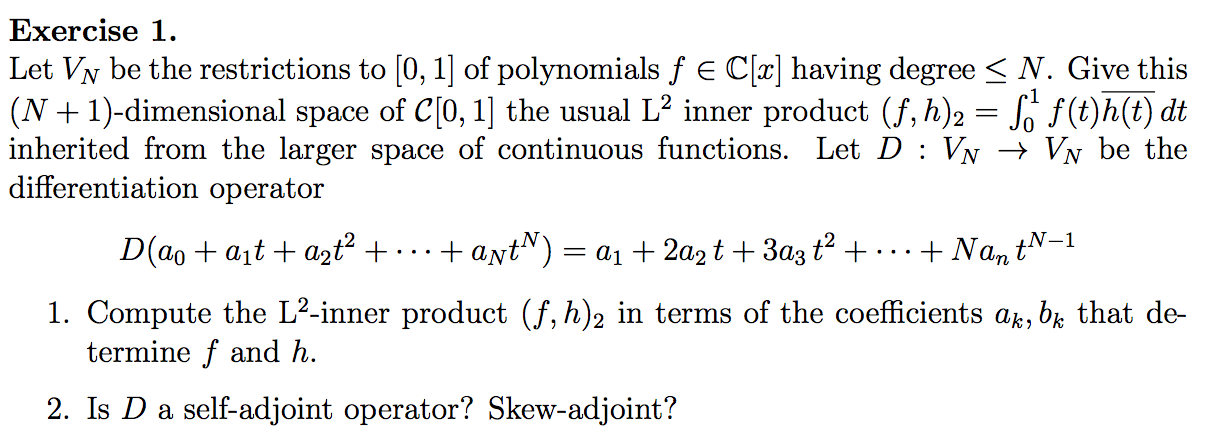
\includegraphics[width=1\textwidth]{LA-1-1.png}
\end{figure}
\end{question}
\begin{solution}
\textbf{(1)} 
By expressing $f,h$ in terms of the coefficients $a_k, b_k$ that determine $f$ and $g$,
exploiting the fact that the complex conjugate of the product is the product of the conjugate,
using the differentiation of complex polynomials, 
we obtain
\eQb
(f,g)_2 &=& 
\int_{0}^{1} (\sum_{i=0}^{N} a_i t^i )\overline{(\sum_{i=0}^{N} b_i t^i)} dt \\ 
&=&  
\int_{0}^{1} (\sum_{i=0}^{N} a_i t^i )(\sum_{i=0}^{N} \overline{b_i}t^i) dt \\
&=& \int_{0}^{1} \sum_{0 \leq i,j \leq N} a_i \overline{b_j} t^{i+j} dt \\
&=& \bigg[ \sum_{0 \leq i,j \leq N} \dfrac{a_i \overline{b_j}}{i+j+1} t^{i+j+1} \bigg]_{0}^{1} \\ 
&=& \sum_{0 \leq i,j \leq N} \dfrac{a_i \overline{b_j}}{i+j+1}. \\
\eQe

\bigskip

\textbf{(2)} By writing down the matrix representation of the differentiation 
operator, using
the standard polynomial basis, $\{ 1, x, x^2, ..., x^n\}$, we see that the matrix does not
equal its conjugate transpose, and also does not equal the negative of the conjugate transpose.
Hence, it is not self-adjoint, and not skew-joint. 
\hfill $\qed$  

\end{solution}

\bigskip

\begin{question}[2]
\hfill
\begin{figure}[h!]
  \centering
    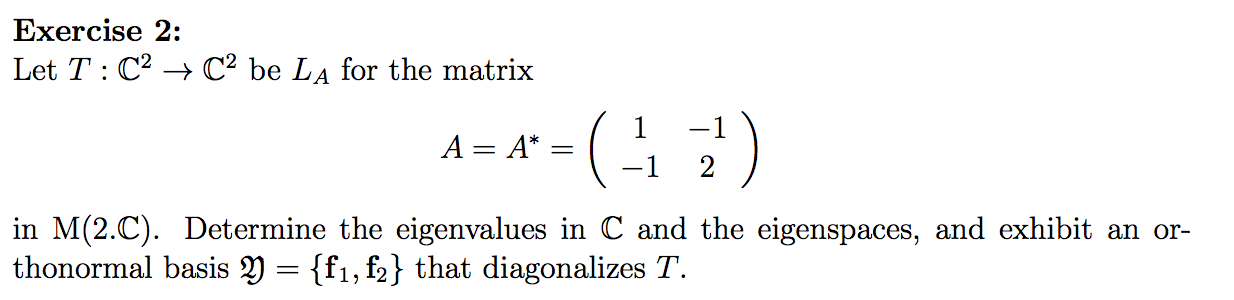
\includegraphics[width=1\textwidth]{LA-1-2.png}
\end{figure}
\end{question}
\begin{solution}
Firstly, the characteristic equation of the matrix $A$ is given by
\eQb
(1-\lambda)(2-\lambda) - 1 &=& 0,
\eQe
which can equivalently written as
\eQb
{\lambda}^2 -3\lambda + 1 &=& 0. 
\eQe
Using the quadratic formula, we obtain that 
$\dfrac{3 \pm \sqrt{5}}{2}$ are the eigenvalues of the matrix. Now, we determine the respective
eigenspaces. 
Recall that we can characterize the 
eigenspace as $\text{Null}(A - \lambda I)$. Hence, for 
 $\lambda = \dfrac{3 + \sqrt{5}}{2}$, we have
\eQb
\text{Null}(A -\lambda I) 
&=& \text{Null} \Big( 
\begin{pmatrix}
1-\dfrac{3 + \sqrt{5}}{2} & -1 \\
-1 & 2 - \dfrac{3 + \sqrt{5}}{2} \\ 
\end{pmatrix} \Big) \\
 &=& \text{Null} \Big( 
\begin{pmatrix}
\dfrac{-1 - \sqrt{5}}{2} & -1 \\
-1 & \dfrac{1 - \sqrt{5}}{2} \\ 
\end{pmatrix} \Big) \\ 
 &=& \text{Span} \Big( 
\begin{pmatrix}
1 \\
\dfrac{-1 - \sqrt{5}}{2} \\ 
\end{pmatrix} \Big), \\
\eQe 
where the last spanning vector is chosen via inspection. Analogously, 
 $\lambda = \dfrac{3 - \sqrt{5}}{2}$, we have
\eQb
\text{Null}(A -\lambda I) 
&=& \text{Null} \Big( 
\begin{pmatrix}
1-\dfrac{3 - \sqrt{5}}{2} & -1 \\
-1 & 2 - \dfrac{3 - \sqrt{5}}{2} \\ 
\end{pmatrix} \Big) \\
 &=& \text{Null} \Big( 
\begin{pmatrix}
\dfrac{-1 + \sqrt{5}}{2} & -1 \\
-1 & \dfrac{1 + \sqrt{5}}{2} \\ 
\end{pmatrix} \Big) \\ 
 &=& \text{Span} \Big( 
\begin{pmatrix}
1 \\
\dfrac{-1 +\sqrt{5}}{2} \\ 
\end{pmatrix} \Big). \\
\eQe
Now, with the eigenspaces computed, we can simply normalize each spanning vector, and obtain the
orthonormal basis that diagnoalizes $T$, which turn out to be $\dfrac{1}{N_1} (1, \dfrac{-1 - 
\sqrt{5}}{2})$ and $\dfrac{1}{N_2} (1, \dfrac{-1-\sqrt{5}}{2})$, where $N_1$ and $N_2$ are the
corresponding normalization scalar. \hfill $\qed$
\end{solution}

\bigskip

\begin{question}[3]
\hfill
\begin{figure}[h!]
  \centering
    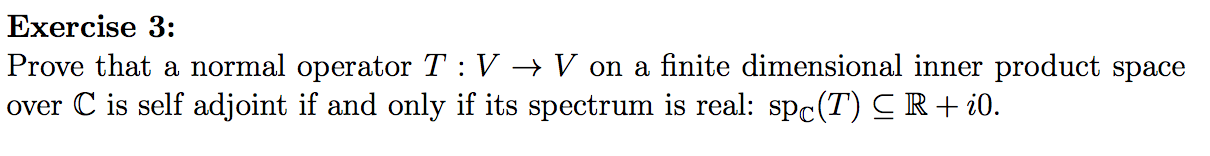
\includegraphics[width=1\textwidth]{LA-1-3.png}
\end{figure}
\end{question}
\begin{solution}
Let $T$ be a normal operator on a finite dimensional inner product space. 
By Complex Spectral theorem, we obtain that $T$ has a diagonal matrix with respect to
some orthonormal basis, which we denote as $M(T)$. By definition, $T$ is self-adjoint iff
$M(T) = M(T)^*$, where $M(T)^*$ denotes the conjugate transpose of $M(T)$. Since, $M(T)$ is 
diagonal, we have that $M(T) = M(T)^*$ iff diagonal entries are real. Since we know that the
diagonal entries of a diagonal matrix is the specturm, we have that the diagonal entries of $M(T)$
is real iff all of its eigenvalues are real. By the chain of equivalence obtained, we are done. 
\hfill $\qed$ 
\end{solution}
\bigskip

\begin{question}[4]
\hfill
\begin{figure}[h!]
  \centering
    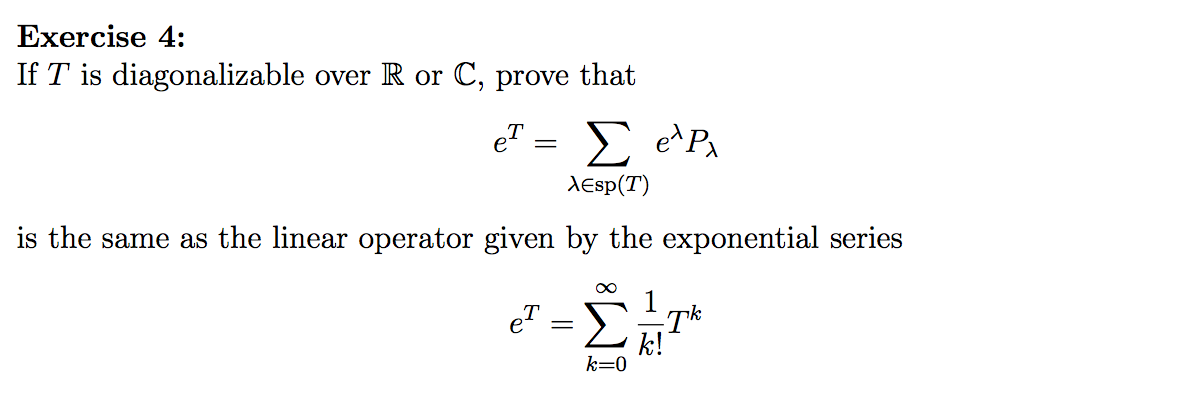
\includegraphics[width=1\textwidth]{LA-1-4.png}
\end{figure}
\end{question}
\begin{solution}
By definition of exponential operator and the given hint, we have
\eQb
e^{T} &=& \sum_{k=0}^{\infty} \dfrac{1}{k!} T^k \\
&=& \sum_{k=0}^{\infty} \dfrac{1}{k!} \sum_{\lambda \in \text{sp}(T)}
 \lambda^k P_{\lambda} \\
&=& \sum_{\lambda \in \text{sp}(T)} \sum_{k=0}^{\infty} \dfrac{\lambda^k}{k!} P_{\lambda} \\
&=& \sum_{\lambda \in \text{sp}(T)} e^{\lambda}P_{\lambda},
\eQe
as $\sum_{k=0}^{\infty} \dfrac{\lambda^k}{k!} = e^{\lambda}$ is a well-known identity in analysis,
and the exchange of the summand is justified by the original convergence. \hfill $\qed$

\end{solution}

\pagebreak

\begin{question}[5]
\hfill
\begin{figure}[h!]
  \centering
    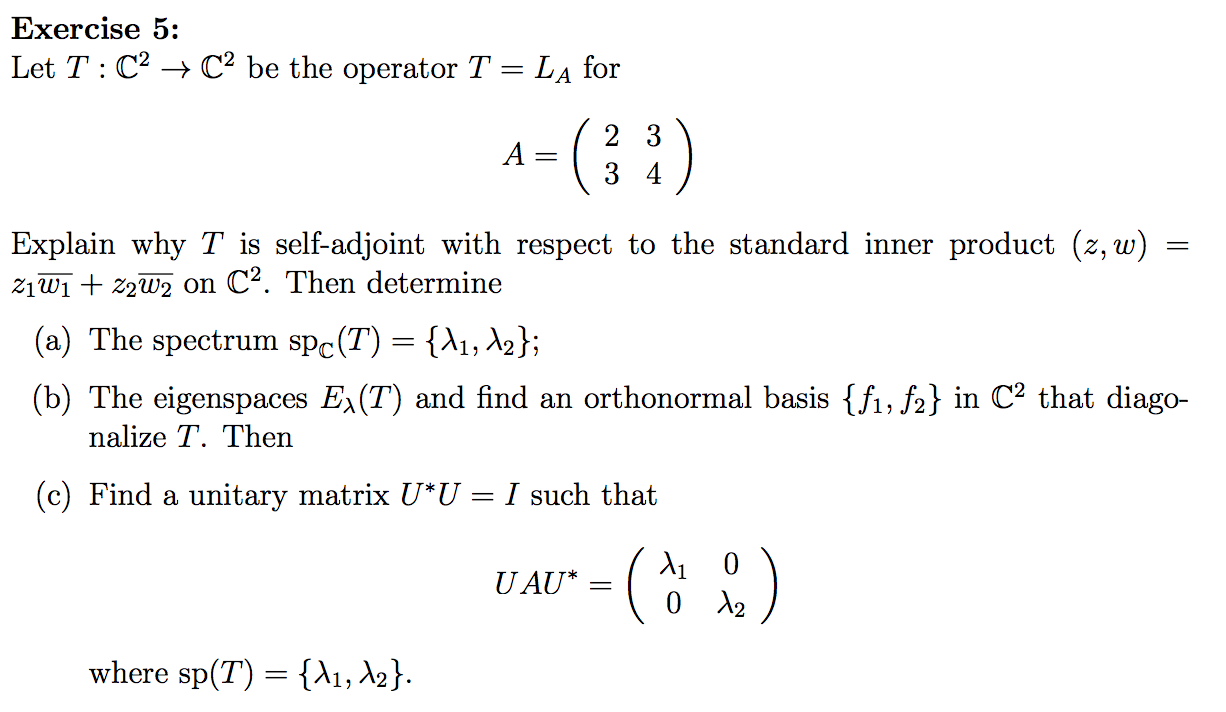
\includegraphics[width=1\textwidth]{LA-1-5.png}
\end{figure}
\end{question}
\begin{solution} Since $L_A$ typically denotes the matrix of an operator, with respect 
to the standard basis, we have that the basis that the matrix is induced by is orthonormal.
In that case, we know that the matrix of the adjoint operator, with respect to the same 
orthonormal basis, is the conjugate transpose of the original matrix. The given matrix equals
its conjugate transpose. Hence, we conclude that it is self-adjoint.

\smallskip

\textbf{(a)}
Firstly, the characteristic equation of the matrix $A$ is given by
\eQb
(2-\lambda)(4-\lambda) - 9 &=& 0,
\eQe
which can equivalently written as
\eQb
{\lambda}^2 -6\lambda - 1 &=& 0, 
\eQe
Using the quadratic formula, we obtain that 
$3 \pm \sqrt{10}$ are the eigenvalues of the matrix. The specturm 
of $A$ is just 
the set formed by those two eigenvalues.

\smallskip

\textbf{(b)} 
Using the same computational step as in the problem 2, we have that the eigenvectors are
$(-1 -\sqrt{10},3)$ and $(-1+\sqrt{10},3)$. As these are linearly independent, one can 
simply normalize them with their respective norms.  

\smallskip

\textbf{(c)} We now have orthonormal bases from $(b)$. The unitary operator $U$ can be formed 
by joining the orthonormal bases column by column. 
\hfill $\qed$

 
\end{solution}

\pagebreak

\begin{question}[6]
\hfill
\begin{figure}[h!]
  \centering
    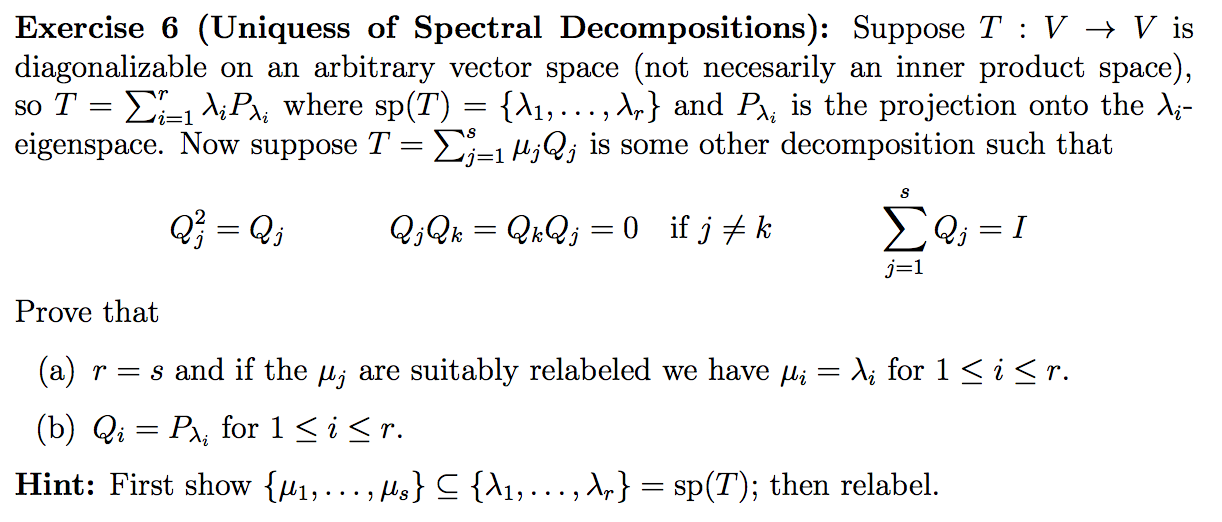
\includegraphics[width=1\textwidth]{LA-1-6.png}
\end{figure}
\end{question}
\begin{solution}
\end{solution}

\end{document}
